
\subsection*{Què és la tecnologia Li-Fi i com funciona?}
\addcontentsline{toc}{subsection}{Què és la tecnologia Li-Fi i com funciona?}

Li-Fi és una forma de comunicació òptica que utilitza la llum visible per a la transmissió de dades. La tecnologia Li-Fi, que significa "Light Fidelity", és un sistema de comunicació sense fil que utilitza llum LED (diodos emissors de llum) per a transmetre dades a una velocitat molt alta. Aquesta tecnologia funciona modulant la intensitat de la llum a una taxa molt ràpida, invisible per a l'ull humà, per transmetre informació.

La tecnologia Li-Fi suposa una gran millora en comparació amb el Wi-Fi a tots els nivells. Per començar, la velocitat de transmissió és fins a 100 vegades més ràpida!

\begin{figure}[h!]
    \centering
    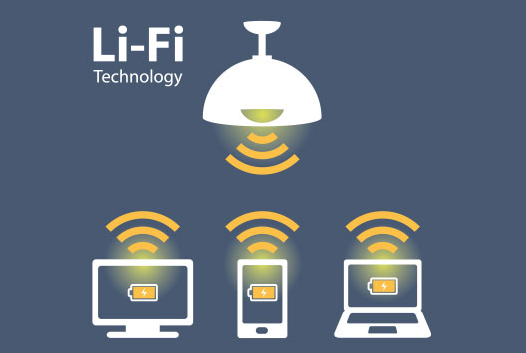
\includegraphics[width=80mm]{lifi.png}
    \caption{visió general de mercat VLC}
    \label{fig:method}
\end{figure}


\subsection*{Sostenibilitat: menor cost i més eficiència}
\addcontentsline{toc}{subsection}{Sostenibilitat: menor cost i més eficiència}

Els seus avantatges no estan només a la velocitat. S'estima que en un futur proper podrem transmetre dades a través de l'energia solar, cosa que facilitarà l'accés a persones sense Internet i amb recursos d'electricitat limitats. El funcionament de la tecnologia Li-Fi estalviarà costos a les llars i, sobretot, als llocs de treball. Podria funcionar sense dispositius electrònics com ara rúters, mòdems, repetidors, amplificadors d'ona i antenes.

Aquests dispositius, que actualment estan connectats a la xarxa elèctrica les 24 hores del dia, els 7 dies de la setmana, deixarien de consumir electricitat i la seva funció seria reemplaçada per una bombeta LED, que en la majoria dels casos ja està encesa durant el horari de treball, per tant, no significaria un cost extra.

La principal diferència entre Li-Fi i altres formes de comunicació òptica, com ara la fibra òptica, és que Li-Fi no utilitza fils físics per a la transmissió de dades. En canvi, transmet les dades mitjançant la il·luminació LED ja existent en un entorn. Aquesta tecnologia pot oferir velocitats de transmissió de dades molt altes i també pot ser utilitzada en entorns on les comunicacions per ones de ràdio poden ser limitades, com ara en hospitals o en aules on l'ús de ones de ràdio pot estar restringit.

\subsection*{Seguridad contra ataques}
\addcontentsline{toc}{subsection}{Seguridad contra ataques}


Al ser necesario estar en contacto directo con el emisor de haz de luz LED, se refuerza la seguridad informática. Solo los dispositivos iluminados por la misma bombilla pueden interconectarse entre sí, eliminando ataques o intentos de entrada no autorizados desde dispositivos fuera de nuestro espectro de luz.

Una solución brillante, más segura, más rápida y eficiente para optimizar nuestra conexión con el mundo.


\subsection*{Incovenients de Li-Fi}
\addcontentsline{toc}{subsection}{Incovenients de Li-Fi}

Encara que la tecnologia Li-Fi ofereix algunes avantatges, també té alguns inconvenients i limitacions que poden afectar la seva adopció i implementació:

\begin{enumerate}
    \item Dependència de la llum visible: La transmissió de dades a través de Li-Fi depèn de la llum visible, de manera que la comunicació pot veure afectada per la falta de llum, com en entorns foscos o quan les llums estan apagades.
    \item Limitacions d'abast: La cobertura de Li-Fi és generalment més limitada que la del Wi-Fi, ja que la llum no penetra a través de parets o altres obstacles com ho fa la radiació de radiofreqüència.
    \item Interferència de la llum solar: La llum solar pot interferir amb la transmissió de dades Li-Fi, ja que les dues fonts de llum poden ser captades pel receptor, provocant interferències i afectant el rendiment de la comunicació.
    \item Limitacions de mobilitat: La tecnologia Li-Fi pot ser menys adequada per a dispositius en moviment, ja que requereix una connexió visual constant amb la font de llum per a una transmissió de dades eficaç.
\end{enumerate}



\subsection*{Productes Li-Fi}
\addcontentsline{toc}{subsection}{Productes Li-Fi}